\section{Komplexe Zahlen}
\begin{mainbox}{Formen \& Operationen}
  $z = x + yi$
    \tiny \color{gray}
      Kartesische Form
    \color{black} \normalsize,
  $\overline{z} = x - iy$
    \tiny \color{gray}
      Konjugation
    \color{black} \normalsize, 
    $i = \sqrt{-1} $ \\
  $|z| = \sqrt{x^2 + y^2} = z \cdot \overline{z}$ 
    \tiny \color{gray}
      Betrag
    \color{black} \normalsize\\
  $z^{-1} = \frac{1}{z} = \frac{\overline{z}}{|z|^2}$, $\forall z \neq 0$
    \tiny \color{gray}
      Reziproke a.k.a. multiplikative Inverses
    \color{black} \normalsize
    
  $+/-: (x_1 + x_2) + (y_1 + y_2) \cdot i$ \\
  $z_1 \cdot z_2 = (x_1 + y_1i) \cdot (x_2 + y_2i) \qquad \frac{z_1}{z_2} = \frac{z_1 \cdot \overline{z_2}}{|z_2|^2}$ \\
\end{mainbox}

\begin{mainbox}{Konjugation}
  $z = x + iy \in \mathbb{C} \longrightarrow \overline{z} = x - iy \in \mathbb{C}$ \\
  Die Konjugation hat die folgenden Eigenschaften
  \begin{itemize}
    \item[i)]  $z \cdot \overline{z} = (x + iy) \cdot (x - iy) = x^2 - i^2 \cdot y^2 \\ = x^2 + y^2 = |z|^2 \Longrightarrow z^{-1} = \frac{\overline{z}}{|z|^2}$, $z \neq 0$
    \item[ii)] $\overline{(z_1 + z_2)} = \overline{z_1} + \overline{z_2}$
    \item[iii)] $\overline{(z_i \cdot z_2)} = \overline{z_1} \cdot \overline{z_2}$
  \end{itemize}
\end{mainbox}

\begin{itemize}[leftmargin=4.5mm, topsep=1pt, itemsep=1pt, parsep=1pt]
    \item Weitere Eigenschaften
    \begin{itemize}[leftmargin=4.5mm, topsep=1pt, itemsep=1pt, parsep=1pt]
      \item[i)] $|z \cdot w| = |z| \cdot |w|$
      \item[ii)] $\left| \frac{z}{w} \right| = \frac{|z|}{|w|}$, $w \neq 0$
      \item[iii)] $|z| = |\overline{z}|$
      \item[iv)] $|z + w| \leqslant |z|$
    \end{itemize} 
  \end{itemize}

\begin{mainbox}{Polarform}
  Die Polarform von $z = x + iy \in \mathbb{C}$ ($\phi \in (- \pi, \pi]$) sei
  $z = r \cdot e^{i \cdot \pi}$ 
    \tiny \color{gray}
      (Euler Form)
    \color{black} \normalsize \\
  $z = r \cdot (\cos(\phi) + i \cdot \sin(\phi))$ 
    \tiny \color{gray}
      (Trigonomical Form)
    \color{black} \normalsize
    \\
    \begin{wrapfigure}[0]{r}{0.25\textwidth}
      \centerline{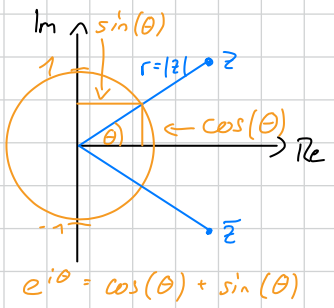
\includegraphics[scale=0.2]{polarform.png}}
      \vspace{10cm}
    \end{wrapfigure}
    mit $r = ||z|| = \sqrt{x^2 + y^2}, x = r \cdot \cos(\phi), y = r \cdot \sin(\phi)$ \\
  $\phi =
  \begin{cases}
    \arctan\left(\frac{y}{x}\right)       & x > 0                      \\
    \arctan\left(\frac{y}{x}\right) + \pi & x < 0 \wedge y \geqslant 0 \\
    \arctan\left(\frac{y}{x}\right) - \pi & x < 0 \wedge y < 0         \\
    \frac{\pi}{2}                         & x = 0  \wedge y > 0        \\
    - \frac{\pi}{2}                       & x = 0 \wedge y < 0         \\
    undefiniert                           & x = 0 \wedge y = 0         \\
  \end{cases}$
\end{mainbox}